% Options for packages loaded elsewhere
\PassOptionsToPackage{unicode}{hyperref}
\PassOptionsToPackage{hyphens}{url}
%
\documentclass[
]{article}
\usepackage{lmodern}
\usepackage{amsmath}
\usepackage{ifxetex,ifluatex}
\ifnum 0\ifxetex 1\fi\ifluatex 1\fi=0 % if pdftex
  \usepackage[T1]{fontenc}
  \usepackage[utf8]{inputenc}
  \usepackage{textcomp} % provide euro and other symbols
  \usepackage{amssymb}
\else % if luatex or xetex
  \usepackage{unicode-math}
  \defaultfontfeatures{Scale=MatchLowercase}
  \defaultfontfeatures[\rmfamily]{Ligatures=TeX,Scale=1}
\fi
% Use upquote if available, for straight quotes in verbatim environments
\IfFileExists{upquote.sty}{\usepackage{upquote}}{}
\IfFileExists{microtype.sty}{% use microtype if available
  \usepackage[]{microtype}
  \UseMicrotypeSet[protrusion]{basicmath} % disable protrusion for tt fonts
}{}
\makeatletter
\@ifundefined{KOMAClassName}{% if non-KOMA class
  \IfFileExists{parskip.sty}{%
    \usepackage{parskip}
  }{% else
    \setlength{\parindent}{0pt}
    \setlength{\parskip}{6pt plus 2pt minus 1pt}}
}{% if KOMA class
  \KOMAoptions{parskip=half}}
\makeatother
\usepackage{xcolor}
\IfFileExists{xurl.sty}{\usepackage{xurl}}{} % add URL line breaks if available
\IfFileExists{bookmark.sty}{\usepackage{bookmark}}{\usepackage{hyperref}}
\hypersetup{
  pdftitle={Gestion de Portefeuille},
  pdfauthor={Patrick Hénaff},
  hidelinks,
  pdfcreator={LaTeX via pandoc}}
\urlstyle{same} % disable monospaced font for URLs
\usepackage[margin=1in]{geometry}
\usepackage{color}
\usepackage{fancyvrb}
\newcommand{\VerbBar}{|}
\newcommand{\VERB}{\Verb[commandchars=\\\{\}]}
\DefineVerbatimEnvironment{Highlighting}{Verbatim}{commandchars=\\\{\}}
% Add ',fontsize=\small' for more characters per line
\usepackage{framed}
\definecolor{shadecolor}{RGB}{248,248,248}
\newenvironment{Shaded}{\begin{snugshade}}{\end{snugshade}}
\newcommand{\AlertTok}[1]{\textcolor[rgb]{0.94,0.16,0.16}{#1}}
\newcommand{\AnnotationTok}[1]{\textcolor[rgb]{0.56,0.35,0.01}{\textbf{\textit{#1}}}}
\newcommand{\AttributeTok}[1]{\textcolor[rgb]{0.77,0.63,0.00}{#1}}
\newcommand{\BaseNTok}[1]{\textcolor[rgb]{0.00,0.00,0.81}{#1}}
\newcommand{\BuiltInTok}[1]{#1}
\newcommand{\CharTok}[1]{\textcolor[rgb]{0.31,0.60,0.02}{#1}}
\newcommand{\CommentTok}[1]{\textcolor[rgb]{0.56,0.35,0.01}{\textit{#1}}}
\newcommand{\CommentVarTok}[1]{\textcolor[rgb]{0.56,0.35,0.01}{\textbf{\textit{#1}}}}
\newcommand{\ConstantTok}[1]{\textcolor[rgb]{0.00,0.00,0.00}{#1}}
\newcommand{\ControlFlowTok}[1]{\textcolor[rgb]{0.13,0.29,0.53}{\textbf{#1}}}
\newcommand{\DataTypeTok}[1]{\textcolor[rgb]{0.13,0.29,0.53}{#1}}
\newcommand{\DecValTok}[1]{\textcolor[rgb]{0.00,0.00,0.81}{#1}}
\newcommand{\DocumentationTok}[1]{\textcolor[rgb]{0.56,0.35,0.01}{\textbf{\textit{#1}}}}
\newcommand{\ErrorTok}[1]{\textcolor[rgb]{0.64,0.00,0.00}{\textbf{#1}}}
\newcommand{\ExtensionTok}[1]{#1}
\newcommand{\FloatTok}[1]{\textcolor[rgb]{0.00,0.00,0.81}{#1}}
\newcommand{\FunctionTok}[1]{\textcolor[rgb]{0.00,0.00,0.00}{#1}}
\newcommand{\ImportTok}[1]{#1}
\newcommand{\InformationTok}[1]{\textcolor[rgb]{0.56,0.35,0.01}{\textbf{\textit{#1}}}}
\newcommand{\KeywordTok}[1]{\textcolor[rgb]{0.13,0.29,0.53}{\textbf{#1}}}
\newcommand{\NormalTok}[1]{#1}
\newcommand{\OperatorTok}[1]{\textcolor[rgb]{0.81,0.36,0.00}{\textbf{#1}}}
\newcommand{\OtherTok}[1]{\textcolor[rgb]{0.56,0.35,0.01}{#1}}
\newcommand{\PreprocessorTok}[1]{\textcolor[rgb]{0.56,0.35,0.01}{\textit{#1}}}
\newcommand{\RegionMarkerTok}[1]{#1}
\newcommand{\SpecialCharTok}[1]{\textcolor[rgb]{0.00,0.00,0.00}{#1}}
\newcommand{\SpecialStringTok}[1]{\textcolor[rgb]{0.31,0.60,0.02}{#1}}
\newcommand{\StringTok}[1]{\textcolor[rgb]{0.31,0.60,0.02}{#1}}
\newcommand{\VariableTok}[1]{\textcolor[rgb]{0.00,0.00,0.00}{#1}}
\newcommand{\VerbatimStringTok}[1]{\textcolor[rgb]{0.31,0.60,0.02}{#1}}
\newcommand{\WarningTok}[1]{\textcolor[rgb]{0.56,0.35,0.01}{\textbf{\textit{#1}}}}
\usepackage{graphicx}
\makeatletter
\def\maxwidth{\ifdim\Gin@nat@width>\linewidth\linewidth\else\Gin@nat@width\fi}
\def\maxheight{\ifdim\Gin@nat@height>\textheight\textheight\else\Gin@nat@height\fi}
\makeatother
% Scale images if necessary, so that they will not overflow the page
% margins by default, and it is still possible to overwrite the defaults
% using explicit options in \includegraphics[width, height, ...]{}
\setkeys{Gin}{width=\maxwidth,height=\maxheight,keepaspectratio}
% Set default figure placement to htbp
\makeatletter
\def\fps@figure{htbp}
\makeatother
\setlength{\emergencystretch}{3em} % prevent overfull lines
\providecommand{\tightlist}{%
  \setlength{\itemsep}{0pt}\setlength{\parskip}{0pt}}
\setcounter{secnumdepth}{-\maxdimen} % remove section numbering
\usepackage[utf8]{inputenc}
\usepackage{float}
\usepackage{eurosym}
\usepackage{booktabs}
\usepackage{longtable}
\usepackage{array}
\usepackage{multirow}
\usepackage{wrapfig}
\usepackage{float}
\usepackage{colortbl}
\usepackage{pdflscape}
\usepackage{tabu}
\usepackage{threeparttable}
\usepackage{threeparttablex}
\usepackage[normalem]{ulem}
\usepackage{makecell}
\usepackage{xcolor}
\ifluatex
  \usepackage{selnolig}  % disable illegal ligatures
\fi

\title{Gestion de Portefeuille}
\usepackage{etoolbox}
\makeatletter
\providecommand{\subtitle}[1]{% add subtitle to \maketitle
  \apptocmd{\@title}{\par {\large #1 \par}}{}{}
}
\makeatother
\subtitle{TP-8: Gestion Obligataire}
\author{Patrick Hénaff}
\date{Février-Mars 2020}

\begin{document}
\maketitle

L'objet de ce TP est de construire un modèle de gestion obligataire qui
combine les méthodes d'adossement flux à flux et d'immunisation.

La méthode d'adossement flux à flux est adaptée aux échéances
court-terme, car elle évite de faire des transactions trop nombreuses.
Par contre, elle manque de flexibilité, et se révèle être une solution
chère. Pour un horizon plus lointain, on lui préfère donc
l'immunisation.

\hypertarget{donnuxe9es}{%
\section{Données}\label{donnuxe9es}}

Les données sont simulées pour les besoins du TP.

\hypertarget{obligations}{%
\subsection{Obligations}\label{obligations}}

\begin{Shaded}
\begin{Highlighting}[]
\NormalTok{df.o }\OtherTok{\textless{}{-}} \FunctionTok{read.csv}\NormalTok{(}\StringTok{"obligations.csv"}\NormalTok{, }
                           \AttributeTok{colClasses=}\FunctionTok{c}\NormalTok{(}\StringTok{"character"}\NormalTok{, }\StringTok{"character"}\NormalTok{, }\ConstantTok{NA}\NormalTok{))}
\NormalTok{df.o}\SpecialCharTok{$}\NormalTok{dtE }\OtherTok{\textless{}{-}} \FunctionTok{as.Date}\NormalTok{(df.o}\SpecialCharTok{$}\NormalTok{dtE, }\FunctionTok{format}\NormalTok{(}\StringTok{"\%m/\%d/\%Y"}\NormalTok{))}
\NormalTok{df.o}\SpecialCharTok{$}\NormalTok{dtM }\OtherTok{\textless{}{-}} \FunctionTok{as.Date}\NormalTok{(df.o}\SpecialCharTok{$}\NormalTok{dtM, }\FunctionTok{format}\NormalTok{(}\StringTok{"\%m/\%d/\%Y"}\NormalTok{))}
\NormalTok{df.o}\SpecialCharTok{$}\NormalTok{name }\OtherTok{\textless{}{-}} \FunctionTok{sapply}\NormalTok{(}\FunctionTok{seq\_along}\NormalTok{(df.o}\SpecialCharTok{$}\NormalTok{dtE), }\ControlFlowTok{function}\NormalTok{(x) }\FunctionTok{paste}\NormalTok{(}\StringTok{\textquotesingle{}Bond{-}\textquotesingle{}}\NormalTok{,x, }\AttributeTok{sep=}\StringTok{\textquotesingle{}\textquotesingle{}}\NormalTok{))}
\FunctionTok{kable}\NormalTok{(df.o[}\DecValTok{1}\SpecialCharTok{:}\DecValTok{10}\NormalTok{,], }
      \AttributeTok{col.names=}\FunctionTok{c}\NormalTok{(}\StringTok{"Dt Emission"}\NormalTok{, }\StringTok{"Dt Maturité"}\NormalTok{, }\StringTok{"Coupon"}\NormalTok{, }\StringTok{"Name"}\NormalTok{),}
      \AttributeTok{format=}\StringTok{"latex"}\NormalTok{, }\AttributeTok{booktabs=}\NormalTok{T)}\SpecialCharTok{\%\textgreater{}\%}
  \FunctionTok{kable\_styling}\NormalTok{(}\AttributeTok{position=}\StringTok{"center"}\NormalTok{)}
\end{Highlighting}
\end{Shaded}

\begin{table}[H]
\centering
\begin{tabular}{llrl}
\toprule
Dt Emission & Dt Maturité & Coupon & Name\\
\midrule
2018-06-01 & 2021-06-01 & 1.7 & Bond-1\\
2016-12-01 & 2021-12-01 & 3.5 & Bond-2\\
2019-04-01 & 2022-04-01 & 1.7 & Bond-3\\
2017-10-01 & 2022-10-01 & 2.6 & Bond-4\\
2020-02-01 & 2023-02-01 & 2.7 & Bond-5\\
\addlinespace
2016-04-01 & 2023-04-01 & 1.2 & Bond-6\\
2018-08-01 & 2023-08-01 & 5.0 & Bond-7\\
2020-12-01 & 2023-12-01 & 2.2 & Bond-8\\
2017-02-01 & 2024-02-01 & 3.5 & Bond-9\\
2019-06-01 & 2024-06-01 & 2.7 & Bond-10\\
\bottomrule
\end{tabular}
\end{table}

\hypertarget{courbe-des-taux-actuariels}{%
\subsection{Courbe des taux
actuariels}\label{courbe-des-taux-actuariels}}

\begin{Shaded}
\begin{Highlighting}[]
\NormalTok{dt.mat }\OtherTok{\textless{}{-}} \FunctionTok{seq}\NormalTok{(}\FunctionTok{ymd}\NormalTok{(}\StringTok{\textquotesingle{}2021{-}01{-}01\textquotesingle{}}\NormalTok{), }\FunctionTok{ymd}\NormalTok{(}\StringTok{\textquotesingle{}2040{-}01{-}01\textquotesingle{}}\NormalTok{), }\AttributeTok{by=}\StringTok{"year"}\NormalTok{)}
\NormalTok{tx }\OtherTok{\textless{}{-}} \DecValTok{1} \SpecialCharTok{+} \FunctionTok{log}\NormalTok{(}\FunctionTok{seq\_along}\NormalTok{(dt.mat))}
\NormalTok{df.cdt }\OtherTok{\textless{}{-}} \FunctionTok{data.frame}\NormalTok{(}\AttributeTok{mat=}\NormalTok{dt.mat, }\AttributeTok{tx=}\NormalTok{tx)}
\FunctionTok{plot}\NormalTok{(dt.mat, tx, }\AttributeTok{type=}\StringTok{\textquotesingle{}l\textquotesingle{}}\NormalTok{, }\AttributeTok{lwd=}\DecValTok{2}\NormalTok{, }\AttributeTok{col=}\StringTok{\textquotesingle{}red\textquotesingle{}}\NormalTok{, }
     \AttributeTok{main=}\StringTok{\textquotesingle{}Courbe des taux actuariels\textquotesingle{}}\NormalTok{,}
     \AttributeTok{xlab=}\StringTok{"Maturité"}\NormalTok{, }\AttributeTok{ylab=}\StringTok{"taux"}\NormalTok{)}
\end{Highlighting}
\end{Shaded}

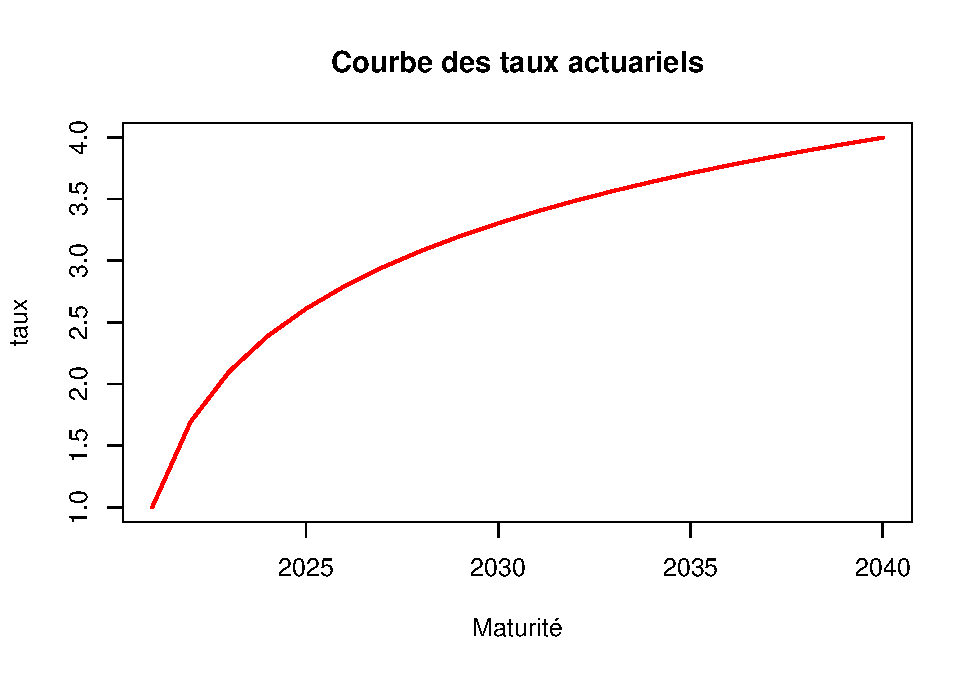
\includegraphics{TP-8_files/figure-latex/unnamed-chunk-2-1.pdf}

\hypertarget{calculs-pruxe9liminaires}{%
\subsection{Calculs préliminaires}\label{calculs-pruxe9liminaires}}

\begin{itemize}
\tightlist
\item
  Ecrire une fonction qui permet d'interpoler la courbe de taux pour une
  date de maturité donnée.
\item
  Choisir une obligation de la liste, interpoler le rendement actuariel
  et calculer le prix ``pied de coupon,'' le coupon couru, le prix
  ``avec coupon couru,'' et les indicateurs de risque. Utiliser le
  paquet ``BondValuation'' et la convention AFB ACT/ACT pour les
  décomptes de jours.
\end{itemize}

\hypertarget{partie-1-immunisation}{%
\section{Partie 1: Immunisation}\label{partie-1-immunisation}}

Soit un passif de 10,000,000\euro~payable le 2/1/2025. Construisez un
portefeuille de deux obligations ayant, au 17/3/2021, la même valeur et
la même PV01 que le passif. Optimisez le rendement moyen du portefeuille
ainsi construit.

\hypertarget{partie-2-plus-difficile-adossement-flux-uxe0-flux-et-immunisation}{%
\section{Partie 2 (plus difficile): Adossement flux à flux et
immunisation}\label{partie-2-plus-difficile-adossement-flux-uxe0-flux-et-immunisation}}

On considère maintenant un passif composé de plusieurs flux, comme
indiqué dans le tableau ci-dessous:

\begin{table}[H]
\centering
\begin{tabular}{lr}
\toprule
Date & Montant\\
\midrule
2021-10-01 & 1e+06\\
2022-04-01 & 1e+06\\
2022-10-01 & 1e+06\\
2023-04-01 & 1e+06\\
2023-10-01 & 1e+06\\
\addlinespace
2024-04-01 & 1e+06\\
2024-10-01 & 1e+07\\
\bottomrule
\end{tabular}
\end{table}

On veut construire un portefeuille de rendement maximum tel que:

\begin{itemize}
\tightlist
\item
  les 4 premiers flux de passif sont adossés
\item
  au 01/04/2023 (date d'immunisation), la PV et PV01 de l'actif et du
  passif sont égales.
\end{itemize}

On suppose que la courbe des taux au 01/04/2023 sera la même qu'au
17/03/2021.

\end{document}
